\subsection{Background} 
  When the project started this year a lot of the fundamental electronics had already been created. This meant that the overall electronic design was decided as well as thrusters and motor-drivers. The power supply was complete as well as the base of the Controller Area Network (CAN) bus. The Microcontroller unit (MCU) AT90CAN128 was decided as a CAN-bus control unit and stacks to mount and connect the cards was complete. There are a lot of redundancy in the system, for example, each CAN-card transforms from 24 to 5V. An explanation for this from the previous team was to increase robustness in the system. If a leakage occurs and the 5V on the power board and 24V is shortened the CAN-card will not burn. Each CAN-card can handle 12.6-48V making them less sensitive to spikes in the system than if one 5V source would go straight in to all of the MCUs.
  
  	\subsubsection{Generic CAN} %Anette
From the previous team, a generic CAN-card was created that has the version number 4.4. This card has nine analogue and eight digital IO-channels. As well as SPI, two UART channels and CAN-bus interface. The card is equipped with a AT90CAN128 MCU giving each card its own computing power. This makes it possible for the card to interpreted CAN-messages, make computation and give out an response. There was a requirement from last year that all of the sensors were to have its own computing power. This requirement was removed during this project. For the most part the card is fully functional. There are some bugs still though. For example the footprint for the 100nF electrolyte capacitor to the left of the switched DC-DC converter is backwards. This can be seen in fig. \ref{Capacitor}

\begin{figure}[!ht]
	\begin{center}
		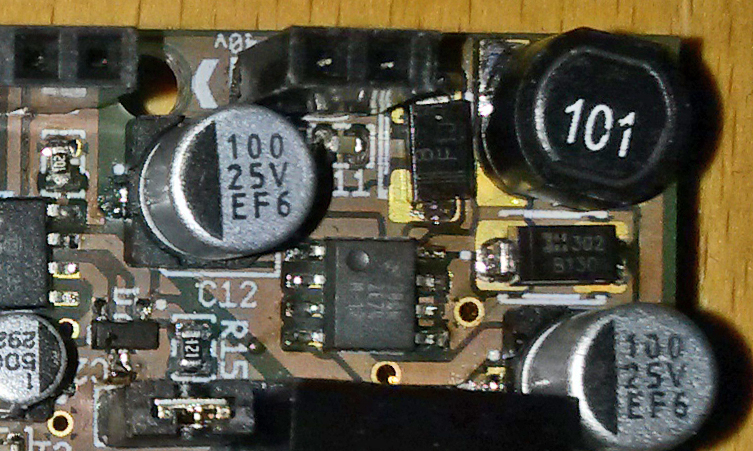
\includegraphics[width=90mm]{./images/Electronics/Capasitor.jpg}
		\caption{The capacitor marked C12 have an incorrect footprint, the footprint is backwards compared to the shoe on the capacitor.}
		\label{Capacitor}
	\end{center}
\end{figure}
   
	\subsubsection{Thrusters} %Patrik
\noindent
The previous team had decided to use the Crustcrawler 400HFS thrusters\cite{thrusters}. They are specially designed for AUV and ROV applications, and are, compared to their size, quite powerful. We had no reason to question this decision since they were already mounted and running. The motors were controlled by the Phoenix Ice2 HV 60 motor controller from Castle Creations \cite{motor_drivers}. The drivers, originally designed for RC air crafts, were bought with custom built firmware, designed to be able to instantly switch rotational direction. The previous team had not been able to get the special firmware settings to work.
 
		\subsubsection{Stack}
	To connect and support the CAN-cards a board that makes it possible to stack these on top of each other was created last year. These holders could hold three cards and the cards was soldered to the stacks. This created some problems with fitting add-on cards. Also if a card would break it was difficult to replace unless all three cards was replaced. 
	
	\subsubsection{Power supply unit} %Anette
A power supply unit (PSU) existed, which was created to supply the different parts of the system from a single source. This card have not been changed during this project. A CAN-card on the PSU can control the supply to different parts of the system. The only thing that can not be control entirely by the software on the CAN card is the supply to the motors. For the thrusters to be supplied the they need to be enabled by the card but the kill-switch also need to activated. The kill switch consists of two physical pins than need to be connected in order to supply the motors. This switch can not be overwritten or controlled in software but are built in to the board. The kill switch controls the power to the thrusters as well as the 12V output but \emph{not} the rest of the system. The CAN-bus and 5V output can be started even if these pins are not connected. There are a few patches on the card printed from Würth electronics. These patches has been added to the schematics but no board design has been made. The schematics is backward constructed from the physical card since proper documentation was absent from the previous group. Even though it has been proofed several times there might still be errors it it. To read more on how the card works see appendix \ref{A_powerboard}. The schematics can be found in appendix \ref{Schematics_Power}.

	\subsubsection{Inertial Navigation System board} %Lennie
When the previous group was working on Naiad the design of the Inertial Navigation System (INS) board was started. A design was proposed for the Fiber Optical Gyroscope (FOG) and was built but not tested. During the summer there was another electronics project where one person had as a mission to test the INS board and discovered that it did not work. The design was not working properly, since the circuit was not complete. Instead it worked as an current generator. A new design was proposed during the summer project and a lot of tips for improving the card was proposed. The proposed board was not built so the design ideas could not be tested. During this years project the ideas was taken into account. Improvements was then made and a new card was built and have been undergoing testing.
	